
\chapter{Grundlagen}
\label{ch:Grundlagen}



\section{SAP}
%SAP SE ist ein deutsches Software-Unternehmen mit Sitz in Walldorf. Als drittgrößter unabhängiger Softwareanbieter der Welt beschäftigt das Unternehmen weltweit mehr als 87 Tausend Mitarbeiter. SAP hat sich vor allem auf Unternehmenssoftware spezialisiert. Einen großen Teil der Firmenaktivitäten bildet die selbst entwickelte ERP Software SAP ERP.\footcite{SAPSE.2017}

ABB nutzt als \ac{ERP}-System die Standardsoftware SAP ECC \footnote{Im weiteren Text nur "`SAP"' genannt} der Firma SAP SE. Eine Standardsoftware ist ein Produkt, welches die allgemeinen Anforderungen des Nutzers - in diesem Fall ABB - erfüllt und bei speziellen Anforderungen individuell angepasst werden kann. Die Firma SAP SE bietet verschiedene modulare Lösungen an, welche einzeln genutzt werden können. Beispiel hierfür sind die \ac{SD}-, \ac{FI}-, \ac{MM}- und \ac{HR}-Module. 

SAP SE hat eigens für ihr \ac{ERP}-System die Programmiersprache \ac{ABAP} entwickelt. Grundsätzlich ist \ac{ABAP} eine Mischung aus \ac{SQL}- und Java-Befehlen. Dabei ist  die Programmiersprache so optimiert, dass effizient mit großen Datenbanken gearbeitet werden kann. In den letzten Jahrzehnten wurde \ac{ABAP} in sofern weiterentwickelt, dass  seit Release 4.6 im Jahre 1999 auch objektorientiertes Arbeiten möglich ist\footnote{Vgl. \cite{Keller.2001} S.16}. Das SAP-System  ist zum größten Teil mit \ac{ABAP} programmiert, sodass Anpassungen und eigene Programme auch in \ac{ABAP} geschrieben werden müssen. 

In dieser Arbeit wird ein Formular erstellt, welches im \ac{GTS}-Modul benutzt wird. Dieses Modul behandelt Prozesse bezüglich gesetzlicher Kontrollen bei In- und Export und deren Zollabwicklung, sowie die in dieser Arbeit behandelte Präferenzabwicklung.




\section{Interactive Forms by Adobe}

Seit 2002 arbeitet SAP SE mit der Software Firma Adobe zusammen, um eine neue Art der Dokumenten-Erstellung im SAP zu schaffen. Aus dieser Zusammenarbeit entstanden die "`Interactive Forms by Adobe"', welche seit Jahren den Standard für die PDF-Erstellung in SAP ERP bilden. Trotz dessen wird diese Technologie bei ABB erst seit einem Jahr eingesetzt.

Neue \ac{PDF}-Dokumente können größtenteils ohne Programmieraufwand erstellt beziehungsweise angepasst werden. Als Hauptwerkzeug dient hierbei der Adobe Lifecycle Designer, welcher mit Hilfe von grafischen Darstellungen einfacheres Arbeiten ermöglicht.\footcite{Bahr.2016}

Die Erstellung von Adobe \ac{PDF}s in SAP besteht aus drei Teilen:

\begin{itemize}
	\item Eine Schnittstelle, in welcher die Daten und Einstellungen der PDF festgelegt sind.
	\item Das eigentliche Formular, welches das Layout sowie den Inhalt des Dokumentes vorgibt.
	\item Ein Druckprogramm, welches die Schnittstelle mit dem Formular verbindet und die PDF druckt.
\end{itemize}

\subsection{Technischer Aufbau der Adobe PDF}
\label{ch:Schnittstelle}

Adobe Forms sind ähnlich unterteilt wie der Vorgänger Smart Forms. Es gibt eine Schnittstelle, in welcher die Datendefinition und die Formularlogik festgelegt werden. Neben den Import- und Export-Parameter für den Dokumentendruck sind auch die tatsächlichen Daten, die das Formular füllen hier definiert. Zusätzlich wird noch die Möglichkeit gegeben, die Daten mit Hilfe von \ac{ABAP}-Code bei der Initialisierung der Dokumentenerstellung anzupassen.

Basierend auf der Schnittstelle gibt es das eigentliche Formular. Jedes Formular muss einer Schnittstelle zugewiesen sein. Nur dann sind die in der Schnittstelle definierten Felder benutzbar. Hier ist zu beachten, dass mehrere Formulare dieselbe Schnittstelle nutzen können. \footnote{Vgl. \cite{Hauser.2015} S.125-128} 

Im Formular wird zuerst ausgewählt, welchen Anteil der Daten, der in der Schnittstelle hinterlegt ist, im Dokument verwendet wird und unter welchen Bedingungen diese ausgegeben werden. Erste Eigenschaften der Felder im Dokument müssen schon hier bestimmt werden wie beispielsweise, ob das Feld aktiv ist oder nicht.


Beim Aktivieren des Formulars wird im Hintergrund ein Funktionsbaustein erstellt, welcher die Schnittstelle zwischen der Datenbeschaffung und Ausgabe des Formulars darstellt. Ein Funktionsbaustein ist ein in sich selbst abgeschlossenes Teilprogramm, welches mit oder ohne Input-Parameter ausgeführt werden kann und mit Hilfe von Export-Parametern Werte zurück gibt. Dieser ist vor allem für Funktionen hilfreich, welche häufig in verschiedenen Programmen in SAP benötigt werden.

\subsection{Aufbau eines Adobe Formulars}
\label{ch:Aufbau}


Die Erstellung eines Dokumentes findet im sogenannten Form Builder statt. Hierbei handelt es sich um ein \ac{GUI} welches die Dokumenterstellung in zwei Teile spaltet - in Kontext und Layout. 

Im Kontext-Bereich stehen die Inhalte der konfigurierten Schnittstelle zur Auswahl. Aus dieser Auswahl wird eine Datenhierarchie festgelegt. Nur diese Inhalte stehen im  Layout zur Verfügung. Sollen bestimmte Bereiche des Dokumentes nur unter definierten Bedingungen angezeigt werden, können diese Einstellungen ebenfalls im Kontext-Bereich vorgenommen werden. Bei manchen Inhalten der \ac{PDF} gibt es Pflichtparameter welche ausgefüllt müssen, zusätzlich zu optional einzustellenden Eigenschaften.
 Elemente der \ac{PDF}, welche beispielsweise abhängig von der Ländersprache sind, müssen einen Wert für die zu verwendete Sprache beinhalten. In Abbildung \ref{figAD} ist dies für das Beispiel der Adressfelder zu sehen. Bei Adressfeldern ist die Ausgabe abhängig vom Absenderland.
 
 \begin{figure}[ht]
 	\centering
 	\makebox[\textwidth][c]{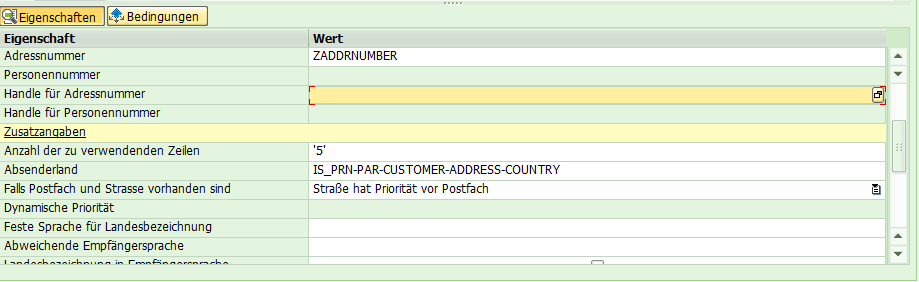
\includegraphics[width=1\textwidth]{img/Adressfeld.png}}%
 	
 	\caption{Eigenschaften eines Adressfeldes}
 	\label{figAD}
 	
 \end{figure}

Unabhängig von den Daten aus der Schnittstelle können zusätzliche Objekte wie Abbildungen und Textbausteine hinzugefügt werden. Der tatsächliche Inhalt dieser Objekte kann wiederum abhängig von den Schnittstellendaten sein. Somit bildet der Kontext-Bereich das Bindeglied zwischen den Formulardaten und dem Dokumentenlayout.\footnote{Vgl. \cite{Hauser.2015} S.145-146} 

Eingebettet in das SAP \ac{GUI} ist der \ac{ALCD}. Mit Hilfe dieses Tools wird die Formularvorlage für den Druck einer Adobe PDF erstellt. Auf Basis der im Kontext definierten Daten wird somit das Layout des Formulars und der anzuzeigenden Inhalt festgelegt. Folgende Funktionen sind hierbei Schlüsselwerkzeuge bei der Erstellung eines Dokumentes: \footcite{Hauser.2015}

\begin{itemize}
	\item Hierarchie und Datenansicht: \\
		Diese zwei baumartigen Darstellungen stellen unterschiedliche Aspekte des Formulars dar. Die Hierarchie zeigt den strukturellen Aufbau des Dokuments, während die Datenansicht den Aufbau der Daten visualisiert.
	\item Bibliothek: \\
		Die Bibliothek bildet eine Sammlung von Feldtypen, welche standardmäßig für ein Dokument zur Verfügung stehen. Oft verwendete Felder, wie beispielsweise Bild- oder Text-Felder, können somit leichter genutzt werden.
	\item Objekt-Palette: \\
		In den verschiedenen Reitern der Objekt-Palette werden die Eigenschaften von Formularfeldern festgelegt.
	\item Formulardesignfläche: \\
		Diese Fläche bildet den Hauptbereich des \ac{ALCD}, da hier die Konfiguration der Formularvorlage stattfindet. Unterteilt wird diese in die Designansicht, welche das Layout und den Inhalt der einzelnen Seiten definiert, sowie die Masterseiten, welche die Hintergründe und das Format der Designseiten vorgibt.
	\item Datenbindungen: \\
		Mit Hilfe der Objekt-Palette wird Feldern eine Datenbindung zugewiesen. Über diese Bindung wird definiert, welche Daten in dem jeweiligen Feld angezeigt werden.
	\item Felder im Fließtext: \\
		Dynamische Inhalte, welche im Fließtext vorkommen, werden mit dieser Funktion eingefügt. Diese Felder werden beim Drucken der PDF gefüllt und der Fließtext wird um das Feld herum dementsprechend angepasst.
	\item Tabellen: \\
		Da die Größe von Tabellen meistens erst zum Zeitpunkt des Druckes feststeht, muss eine dynamische Ausgabe ermöglicht werden. Mit dieser Funktion können Tabellen erstellt und die Ausgaberegeln festgelegt werden.
	\item Seitenumbrüche: \\
		Bei Dokumenten mit dynamischen Inhalten ist es mit Hilfe dieser Funktion möglich, bedingte Seitenumbrüche festzulegen, um gegebenenfalls Inhalte auf einer beliebigen Anzahl neuer Seiten mit einem festgelegten Layout darzustellen.
\end{itemize} 
       
Adobe Forms können zusätzlich dazu benutzt werden, interaktive Formulare zu erstellen. Diese \ac{PDF}s können Elemente enthalten, welche nach dem Druck ausgefüllt werden können. Hierbei ist es möglich Auswahlfelder zu erstellen beziehungsweise den Aufbau des Dokuments dynamisch an die Eingaben anzupassen. Diese interaktive Funktionen werden in dieser Arbeit nicht weiter ausgeführt.
\FloatBarrier
\section{Langzeit-Lieferantenerklärung}
\label{LLE}

 Lieferantenerklärungen sind Dokumente, welche bei einer Lieferung Auskunft bezüglich des Herkunftslandes der gelieferten Materialien gibt. Diese Herkunftsangaben sind Voraussetzung für die Inanspruchnahme einer Zollpräferenz. Diese Zollpräferenz reduziert den Zollsatz für ein präferenzberechtigtes Material, in der Regel, auf null Prozent.\footnote{Vgl. \cite{Schnellenbach.2015} S. 351} Grundsätzlich findet die \ac{LE} bei Warenbewegungen innerhalb der \ac{EU} Anwendung. Die \ac{LLE}, welche als Beispiel-Dokument für diese Arbeit verwendet wird, ist eine einmalige Erklärung, welche für gleiche Lieferungen über einen maximalen Zeitraum von zwei Jahren gilt.\footnote{Vgl. \cite{ZOLL.2017}} 2016 erstellte ABB alleine in Deutschland dieses Dokument 1800 mal.\footnote{Diese Anzahl war das Ergebnis eines intern entwickelten Reports, welcher die ausgedruckten Dokumente im SAP gezählt hat} Text und Aufbau der Lieferantenerklärung entsprechen gesetzlichen Vorgaben. Dementsprechend wird in der folgenden Arbeit nur auf die technische Umsetzung eingegangen.
